%%% Preamble
\documentclass[paper=a4, fontsize=11pt]{scrartcl}
\usepackage[utf8]{inputenc}
\usepackage[T1]{fontenc}
\usepackage{fourier}
\usepackage[french]{babel}
\usepackage[protrusion=true,expansion=true]{microtype}	
\usepackage{amsmath,amsfonts,amsthm} % Math packages
\usepackage[pdftex]{graphicx}	
\usepackage{url}
\usepackage{pdfpages}
\usepackage{todonotes}
\usepackage[a4paper, body={17cm,24cm}]{geometry}


%%% Custom sectioning
\usepackage{sectsty}
\allsectionsfont{  \normalfont\scshape}
%\allsectionsfont{\centering \normalfont\scshape}

%%% Custom headers/footers (fancyhdr package)
\usepackage{fancyhdr}
\pagestyle{fancyplain}
\fancyhead{}											% No page header
\fancyfoot[L]{}											% Empty 
\fancyfoot[C]{}											% Empty
\fancyfoot[R]{\thepage}									% Pagenumbering
\renewcommand{\headrulewidth}{0pt}			% Remove header underlines
\renewcommand{\footrulewidth}{0pt}				% Remove footer underlines
\setlength{\headheight}{13.6pt}


%%% Equation and float numbering
\numberwithin{equation}{section}		% Equationnumbering: section.eq#
\numberwithin{figure}{section}			% Figurenumbering: section.fig#
\numberwithin{table}{section}				% Tablenumbering: section.tab#


%%% Define new commands
\newcommand{\horrule}[1]{\rule{\linewidth}{#1}} 	% Horizontal rule
\renewcommand{\bf}[1]{\textbf{#1}}
\renewcommand{\it}[1]{\textit{#1}}

\newcommand{\Todo}[1]{\todo[inline]{#1}}

\usepackage{color}
\usepackage{xcolor}

\usepackage{caption}
\DeclareCaptionFont{white}{\color{white}}
\DeclareCaptionFormat{listing}{\colorbox{gray}{\parbox{\textwidth}{#1#2#3}}}
\captionsetup[lstlisting]{format=listing,labelfont=white,textfont=white}

\usepackage[numbered]{mcode}

\lstset{breaklines=true,columns=fullflexible}


%%% Begin document
\begin{document}
\includepdf[pages={1}]{title.pdf}

\tableofcontents
\listoftodos

\newpage

%%%%%%%%%%%%%%%%%%%%%%%%%%%%%%%%%%%%%%%%%%%%%%%%%%%%%%%%%%%%%%%%%%%%%%%%%%%%%%%%%%%%%%%%%%%%%%%%%%%%%%%%%%%%%%%%%%%%%%%%%%%
%%%%%%%%%%%%%%%%%%%%%%%%%%%%%%%%%%%%%%%%%%%%%%%%%%%%%%%%%%%%%%%%%%%%%%%%%%%%%%%%%%%%%%%%%%%%%%%%%%%%%%%%%%%%%%%%%%%%%%%%%%%
%%%%%%%%%%%%%%%%%%%%%%%%%%%%%%%%%%%%%%%%%%%%%%%%%%%%%%%%%%%%%%%%%%%%%%%%%%%%%%%%%%%%%%%%%%%%%%%%%%%%%%%%%%%%%%%%%%%%%%%%%%%
\section{\'Etude des problèmes soumis par les responsables}
Cette section traite de la résolution des problèmes soumis par les différents acteurs de l'entreprise. Chaque sous-section aborde un problème et tente de proposer une solution optimale plausible pour ce dernier.

%%%%%%%%%%%%%%%%%%%%%%%%%%%%%%%%%%%%%%%%%%%%%%%%%%%%%%%% NOTATIONS %%%%%%%%%%%%%%%%%%%%%%%%%%%%%%%%%%%%%%%%%%%%%%%%%%%%%%%%
\subsection*{Notations}

Dans le document suivant, nous allons utiliser : 
$A$, $B$, $C$, $D$, $E$ et $F$ pour désigner les différents produits $P_i$. Les quantités respectives $q_i$ seront désignées par $q_A$, $q_B$, $q_C$, $q_D$, $q_E$ et $q_F$. Le prix de vente du produit $P_i$ sera noté $p_i$. Le coût de production du produit $P_i$ sera noté $c_i$, le coût de production comprends le coût des matières premières et le coût de fabrication dû aux machines.

%%%%%%%%%%%%%%%%%%%%%%%%%%%%%%%%%%%%%%%%%%%%%%%%%%%%%%%% COMPTABLE %%%%%%%%%%%%%%%%%%%%%%%%%%%%%%%%%%%%%%%%%%%%%%%%%%%%%%%%
\subsection{Comptable}
\bf{Problème soumis :}
Le problème soumis par le comptable est le suivant, celui-ci souhaite maximiser les bénéfices de l'entreprise.\\

\bf{Solution proposée :}

On a cherché à maximiser le bénéfice que l'on a exprimé, 

\[f(Q) = (\sum_i q_i \times p_i ) - (\sum_i q_i \times c_i) \quad \text{  avec } \, Q, \, \text{ vecteur des quantités } \, q_i \]

ce qui nous donne pour chaque produit la quantité hebdomadaire à produire :
\begin{center}
\begin{tabular}{cccccc}
\hline
$q_A$ & $q_B$ & $q_C$ & $q_D$ & $q_E$ & $q_F$ \\
\hline
5,83 & 11,61 & 12,16 & 1,3 & 31,65 & 27,48 \\
\hline
\end{tabular}
\end{center}

On remarque que le produit E est le plus rentable, puis le produit F, puis C, puis B, puis A et enfin D. De ce fait, il faut favoriser la production des produits en suivant cet ordre. Ce qui explique que le produit E est celui qui doit être le plus produit et le produit D est celui qui doit être le moins produit.

%%%%%%%%%%%%%%%%%%%%%%%%%%%%%%%%%%%%%%%%%%%%%%%%%%%%%%%% RESP ATELIER %%%%%%%%%%%%%%%%%%%%%%%%%%%%%%%%%%%%%%%%%%%%%%%%%%%%%%%%

\subsection{Responsable d'atelier}
\bf{Problème soumis :}

Le problème soumis par le responsable de l'atelier est le suivant, ce dernier souhaite maximiser la quantité totale de produits fabriqués. De ce fait, la fonction à maximiser ne devra pas favoriser un type de produit par rapport à un autre.\\

\bf{Solution proposée :}

On cherche de ce fait à maximiser l'équation (en tenant des comptes des contraintes):

\[f(Q) = \sum_i q_i \quad \text{  avec } \, Q, \, \text{ vecteur des quantités } \, q_i \]

\bf{Résultat :}

Le résultat de l'étude est le suivant : 

\begin{center}
\begin{tabular}{cccccc}
\hline 
$q_A$ & $q_B$ & $q_C$ & $q_D$ & $q_E$ & $q_F$ \\ 
\hline 
5 & 34,64 & 38,85 & 0 & 181,71 & 98,43 \\ 
\hline 
\end{tabular} 
\end{center}

On constate donc qu'il ne faut pas fabriquer de produits D si l'on souhaite maximiser le nombre de produits à fabriquer. Ceci n'est cependant pas une solution qui sera compatible avec les autres responsables. En effet, il y a un déséquilibre important entre la production de produit $A$ et $E$, ce qui ne conviendra pas au responsable commercial.

Cette étude permet de trouver la quantité maximale de produit qui peut être produite par l'entreprise.
\[ Q_{max} = 378,6 \text{ produits}\]

Cette limite supérieure présente l'intérêt de proposer intervale de recherche pour d'autres études.


%%%%%%%%%%%%%%%%%%%%%%%%%%%%%%%%%%%%%%%%%%%%%%%%%%%%%%%% RESP DES STOCK %%%%%%%%%%%%%%%%%%%%%%%%%%%%%%%%%%%%%%%%%%%%%%%%%%%%%%%%
\subsection{Responsable des stocks}
\bf{Problème soumis :}

Le responsable des stocks souhaite quant à lui minimiser la quantité de matière stockée (qu'elle soit brute ou transformée).\\

Ainsi on doit donc minimiser la quantité de produits stockés (c'est-à-dire à minimiser $q_a + q_b + q_c + q_d + q_e + q_f$, ainsi que les matières premières stockées (soit $4q_a + 4q_b + 5q_c + 9q_d + 4q_e + 3q_f$).
\\

\bf{Solution proposée :}

On souhaite donc minimiser la fonction suivante : 

\[ f(Q) = 5q_a + 5q_b + 6q_c + 10q_d + 5q_e + 4q_f \]

Cependant, sans contrainte supplémentaire, on se place dans le cas irréaliste où l'on pourrait diminuer d'autant que l'on souhaite le nombre de produits fabriqués par l'entreprise.\\
Il faut donc ajouter une contrainte, qui peut être une contrainte sur un nombre minimal de produits à fabriquer, ou bien sur le bénéfice souhaité par exemple.\\
Pour l'étude, il a été fixé un nombre minimal de produit à fabriquer. Nous avons fait varier ce nombre pour voir s'il n'y a pas un "sweet spot".

\bf{Résultat :}

Le résultat de l'étude est le suivant : 

\begin{figure}[hbtp]
\caption{Nombre de produits en fonction du stock total \label{figstock}}
\centering
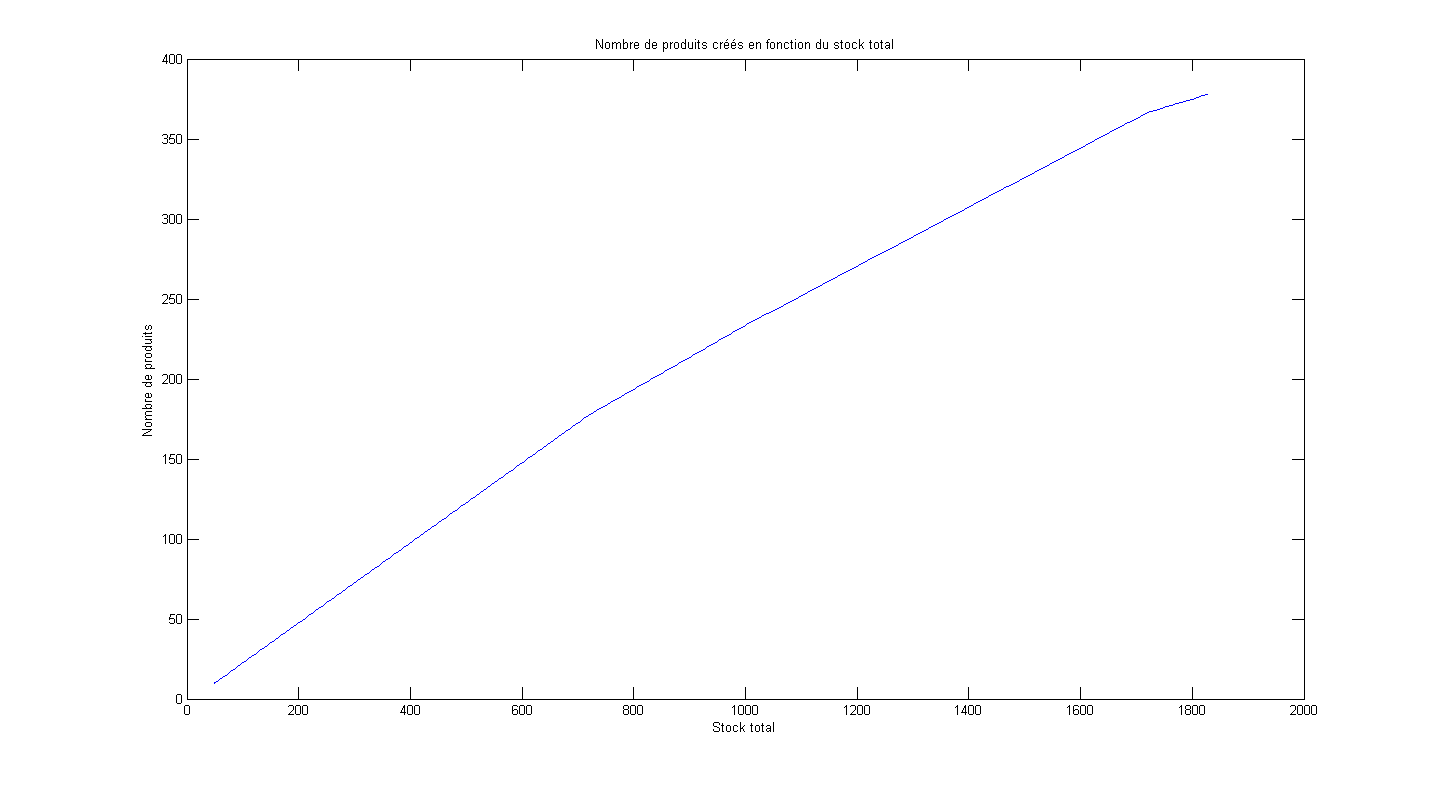
\includegraphics[width=16cm]{figures/nbProduitsFctStockTotal.png}
\end{figure}

\begin{figure}[hbtp]
\caption{Variation du coefficient de la courbe de la figure \ref{figstock}}
\centering
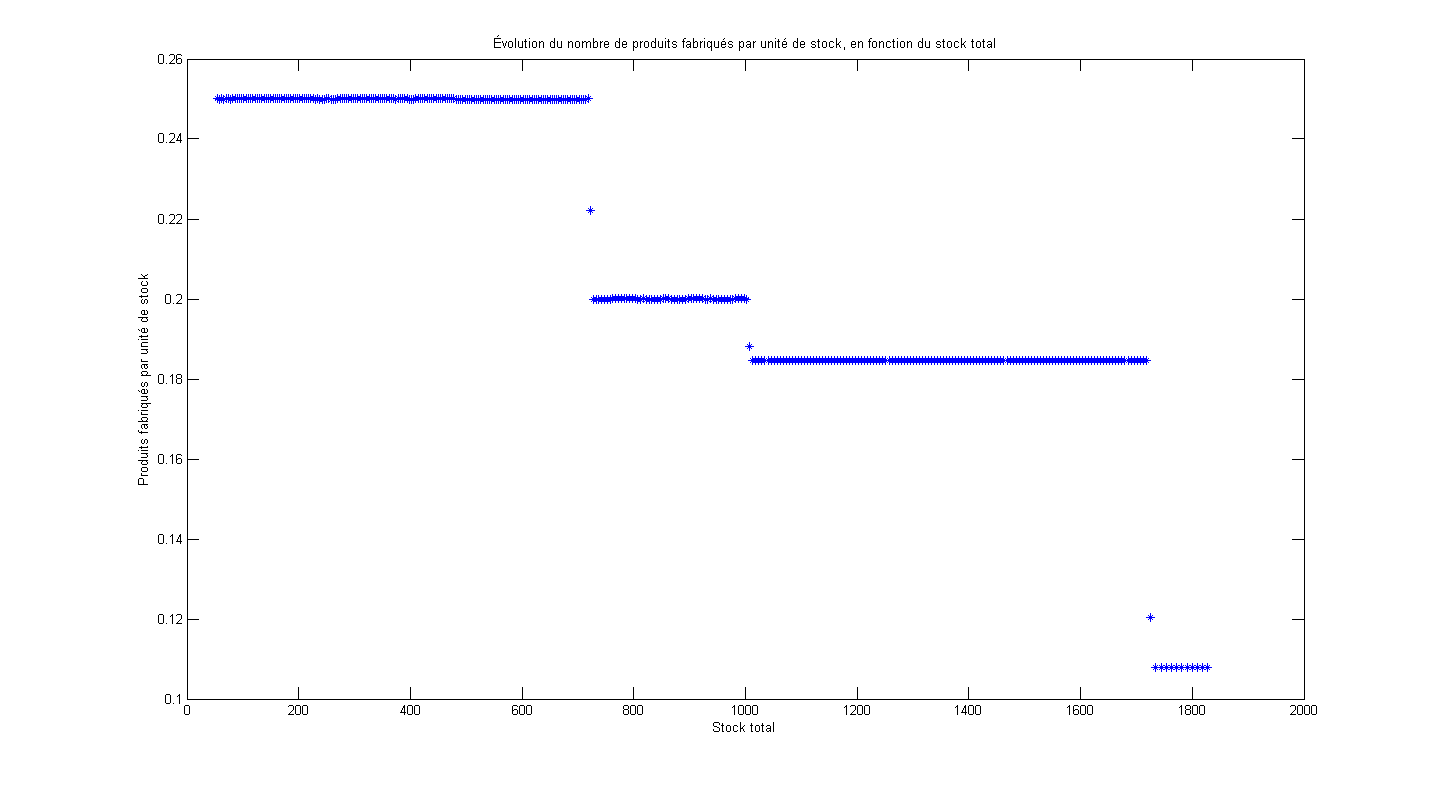
\includegraphics[width=16cm]{figures/nbProduitsFctStockTotal_Coeff.png}
\end{figure}


Etant donné que la figure \ref{figstock} ne montre pas d'endroit où il y aurait un stock idéal en fonction du nombre de produits, nous pouvons choisir arbitrairement, bien qu'en tenant compte des résultats précédents, d'une production de 300 produits. 

La répartition serait alors : 

\Todo{utiliser Matlab pour avoir une répartition du stock pour 300 produits en fabrication par semaine}
\begin{center}
\begin{tabular}{cccccc}
\hline 
$q_A$ & $q_B$ & $q_C$ & $q_D$ & $q_E$ & $q_F$ \\ 
\hline 
5 & 34,64 & 38,85 & 0 & 181,71 & 98,43 \\ 
\hline 
\end{tabular} 
\end{center}



%%%%%%%%%%%%%%%%%%%%%%%%%%%%%%%%%%%%%%%%%%%%%%%%%%%%%%%% RESP COMMERCIAL %%%%%%%%%%%%%%%%%%%%%%%%%%%%%%%%%%%%%%%%%%%%%%%%%%%%%%%%
\subsection{Responsable commercial}
\bf{Problème soumis :}

Le responsable commercial souhaite pour sa part équilibrer la quantité de produite des produits A et E.\\

\bf{Solution proposée :}

Suite à notre étude du problème, c'est à dire la maximisation des bénéfices en équilibrant la production des produits A et E, plusieurs constats peuvent être faits :\\
Pour un écart nul entre les quantités de A et E produites on a les quantités hebdomadaires suivantes suivants :
\begin{center}
\begin{tabular}{cccccc}
\hline
$q_A$ & $q_B$ & $q_C$ & $q_D$ & $q_E$ & $q_F$ \\
\hline
119.08 & 6.91 & 42.58 & 0.00 & 119.08 & 87.24 \\
\hline
\end{tabular}
\end{center}
Tout d'abord le produit D ne semble pas rentable car l'étude conclue qu'il serait optimal de ne plus le produire du tout.
On remarque également que l’évolution de e tend à favoriser la production du produit E plutôt que le produit A.

%%%%%%%%%%%%%%%%%%%%%%%%%%%%%%%%%%%%%%%%%%%%%%%%%%%%%%%% RESP DU PERSONNEL %%%%%%%%%%%%%%%%%%%%%%%%%%%%%%%%%%%%%%%%%%%%%%%%%%%%%%%%
\subsection{Responsable du personnel}
\bf{Problème soumis :}

Le responsable du personnel souhaite minimiser le temps d'utilisation de la machine 4.\\

\bf{Solution proposée :}

%%%%%%%%%%%%%%%%%%%%%%%%%%%%%%%%%%%%%%%%%%%%%%%%%%%%%%%%%%%%%%%%%%%%%%%%%%%%%%%%%%%%%%%%%%%%%%%%%%%%%%%%%%%%%%%%%%%%%%%%%%%%%%%%
%%%%%%%%%%%%%%%%%%%%%%%%%%%%%%%%%%%%%%%%%%%%%%%%%%%%%%%% RESP DES STOCK %%%%%%%%%%%%%%%%%%%%%%%%%%%%%%%%%%%%%%%%%%%%%%%%%%%%%%%%
%%%%%%%%%%%%%%%%%%%%%%%%%%%%%%%%%%%%%%%%%%%%%%%%%%%%%%%%%%%%%%%%%%%%%%%%%%%%%%%%%%%%%%%%%%%%%%%%%%%%%%%%%%%%%%%%%%%%%%%%%%%%%%%%
\section{\'Etude du problème soumis par le Responsable de l'entreprise}

\newpage

\section{Listing - Scripts Matlab}

\lstlistoflistings

\lstinputlisting[caption=Comptable]{scripts/Comptable.m}
\lstinputlisting[caption=Responsable Atelier]{scripts/ResponsableAtelier.m}
\lstinputlisting[caption=Responsable Commercial]{scripts/ResponsableCommercial.m}
\lstinputlisting[caption=Responsable Stocks]{scripts/ResponsableStock.m}
\lstinputlisting[caption=Responsable Personel]{scripts/ResponsablePersonnel.m}

%%% End document
\end{document}
